

\documentclass[12pt]{article} % use larger type; default would be 10pt

\usepackage{enumerate}
\usepackage{graphicx} 
\usepackage{framed}
\usepackage{multicol}


\title{Hibernia College}
\author{Kevin O'Brien}

\begin{document}


\begin{center}
\huge{Mathematics for Computing}\\
\LARGE{Mock Exam 2015}
\end{center}

%---------------------------------------%
\subsection*{Question 1}

\begin{enumerate}[(i)]
	\item (1 Mark) When is the positive integer $p$ said to be a prime number?
	\item (2 Marks) Express the following hexadecimal number as a decimal number, and as a binary number: \[(A32.8)_{16}\]
	
	\item (2 Marks) Convert the following decimal number into base 2, showing all your working:
	$(253)_{10}$. 
		\item (2 Marks) Covert the decimal integer $(407)_{10}$ to binary notation.
		
		\item (2 Marks) Showing your working, express the following number 
		\[ 1.024024024024\ldots\]
		as a ration number in its simplest form.
	\item (1 Mark) Compute the following $101101_2 + 1101_2$ 
\end{enumerate}
%--------------------------------------------------- %
\subsection*{Question 2}
%Question 2
Let A and B and C be subsets of a universal set U.
\begin{itemize}
\item[(a)] (1 Mark) Draw a labelled Venn diagram depicting A,B,C in such a way that they divide
U into 8 disjoint regions. [1]
\item[(b)] (3 Marks) The subset $X \subseteq U$ is defined by the following membership table below. Shade the region X on your diagram. Describe the region you have shaded in
set notation as simply as you can. 
\end{itemize}
{\LARGE
\begin{center}
\begin{tabular}{|c|c|c|c|}
	\hline
	A & B & C & X \\ \hline
	0 & 0 & 0 & 0 \\ \hline
	0 & 0 & 1 & 1 \\ \hline
	0 & 1 & 0 & 0 \\ \hline
	0 & 1 & 1 & 0 \\ \hline
	1 & 0 & 0 & 1 \\ \hline
	1 & 0 & 1 & 1 \\ \hline
	1 & 1 & 0 & 1 \\ \hline
	1 & 1 & 1 & 0 \\ \hline
\end{tabular} 
\end{center}
}
\begin{itemize}
\item[(c)] (3 Marks) The subset $Y \subseteq U$ is defined as $Y = A \cup (C − B)$. Construct the membership
table for Y. 
\item[(d)] (3 Marks) For each of the following statements say whether it is true or false, justifying
your answer, using the Venn diagram you drew earlier.

\begin{enumerate}[(i)]
\item $Y \subseteq X$
\item $Y^{\prime} \subseteq X^{\prime}$
\item $Y − X = A \cap B \cap C$.
\end{enumerate}
\end{itemize}
%=====================================================================%
\subsection*{Question 3}
%2003

\begin{itemize}
\item[(a)] Let n be an element of the set $\{10, 11, 12, 13, 14, 15, 16, 17, 18, 19\}$,
and p and q be the propositions:
\[p : n \mbox{ is odd},   q : n < 15\]. Draw up truth tables for the following statements and find the values of n for
which they are true:
\begin{itemize}
\item[(i)] $ p \vee \neg q$ 
\item[(ii)] $\neg p \wedge q$
\end{itemize}
\item[(b)] Use truth tables to find a statement that is logically equivalent to $\neg p \rightarrow q$.
\end{itemize}

%--------------------- %
% - 1.2 2010 
\begin{enumerate}[(i)]
\item
\end{enumerate}
%=====================================================================%
\subsection*{Question 4}
Let $S$ be the set of all 4 bit binary strings. The function $f : S \rightarrow Z$
is defined by the rule:
\[f(x) = \mbox{ the number of zeros in x} \] for each binary string $x \in S$.
Find:
\begin{itemize}
	\item[(a)] (4 Marks) Answer the following questions
\begin{itemize}
\item[(i)] the number of elements in the domain
\item[(ii)] f(1010)
\item[(iii)] the set of pre-images of 1
\item[(iv)] the range of f. 
\end{itemize}
\item[(b)] (2 Marks) Decide whether the function $f$, as defined above, has either the one to one or
the onto property, justifying your answers. 
\item[(c)] (2 Marks) State the condition to be satisfied by a function $f : X \rightarrow Y$ for it to have an
inverse function $f^{−1} : Y \rightarrow X$.
\item[(d)] (2 Marks) Define the inverse functions for each of the following:
\end{itemize}
%---------------------------------------------------------%
\section*{Question 5}

\begin{figure}
\centering
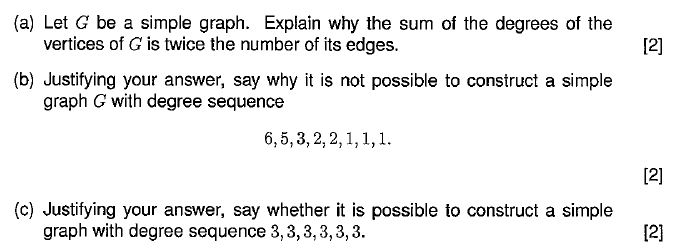
\includegraphics[width=0.7\linewidth]{GraphTheoryQuestion2012}

\end{figure}

\section*{Question 5}
Given the following definitions for simple, connected graphs:
\begin{itemize}
	\item $K_n$ is a graph on $n$ vertices where each pair of vertices is connected by an edge;
	\item $C_n$ is the graph with vertices $v_1, v_2, v_3, \dots, v_n$ and edges $\{v_1,v_2\}, \{v_2,v_3\}, \dots\{v_n, v_1\}$;
	\item $W_n$ is the graph obtained from $C_n$ by adding an extra vertex,$v_{n+1}$, and edges
	from this to each of the original vertices in $C_n$.
\end{itemize}
(a) Draw $K_4$, $C_4$, and $W_4$. 

%----------------------------- %
% 2006 
a) (i) A simple, connected graph has 7 vertices, all having the same degree d.
State the possible values of d and for each value also give the number of edges
in the corresponding graph.
(ii) Another simple, connected graph has 6 vertices, all having the same degree,
n. Draw such a graph when n = 3 and state the other possible values of n.
[4]
%----------------------------------------------------------------%
\newpage
\section*{Question 6}
% 2007 Q8
Given a flock of chickens, between any two chickens one of them is
dominant. A relation, R, is defined between chicken x and chicken y as xRy if x is
dominant over y. This gives what is known as a pecking order to the flock. Home
Farm has 5 chickens: Amy, Beth, Carol, Daisy and Eve, with the following relations:

\begin{itemize}
	\item Amy is dominant over Beth and Carol
	\item Beth is dominant over Eve and Carol
	\item Carol is dominant over Eve and Daisy
	\item Daisy is dominant over Eve, Amy and Beth
	\item Eve is dominant over Amy.
\end{itemize}

\newpage
\section*{Question 6}
% Digraphs and Relations
% http://staff.scem.uws.edu.au/cgi-bin/cgiwrap/zhuhan/dmath/dm_readall.cgi?page=20

Let $A=\{0,1,2\}$ and $R=\{ (0,0),(0,1),(0,2),(1,1), (1,2), (2,2)\}$
and $S=\{(0,0),(1,1),(2,2)\}$ be 2 relations on A. Show that

\begin{itemize}
	\item[(i)] R is a partial order relation.
	\item[(ii)] S is an equivalence relation.
\end{itemize}
%---------------------------------------------------------------------------%

%2002 Question 7
Let S be a set and let R be a relation on S
Explain what it means to say thet $\mathcal{R}$ is

\begin{itemize}
	\item[(i)] reflexive
	\item[(ii)] symmetrix
	\item[(iii)] anti-symmetric
	\item[(iv)] Transitive
	%---------------------------------------------------------------------------%
	
	
	
\end{itemize}


%--------------------------------------------------------------------------- %
\section*{Question 7}
Let the sequence un be defined by the recurrence relation
\[u_{n+1} = u_n + 2n, \mbox{ for n = 1, 2, 3, ...}\]
and let $u_1 = 1$.\\
\begin{figure}[h!]
\centering
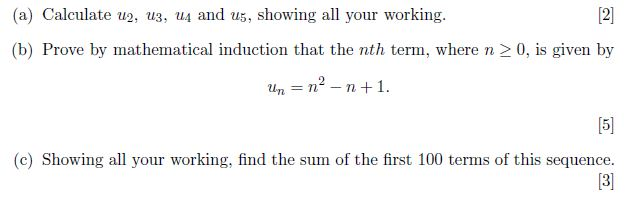
\includegraphics[width=1.11\linewidth]{SeqSerQuestion2005}
\end{figure}

%---------------------------------------------------------------------------%
% TREES
\newpage
\section*{Question 8}
\noindent \textbf{(Part A : Spanning Trees -  5 Marks) }\\
\begin{figure}[h!]
\centering
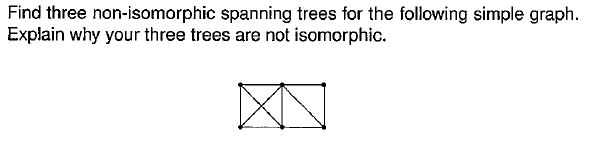
\includegraphics[width=1.11\linewidth]{TreesQuestion2012}
\end{figure}

%	Question 8A
%	\begin{enumerate}
%		\item How many edges are in the spanning tree $T$ ?
%		\item What is the sum of the degree sequence of $T$?
%		\item Write down all the possible degree sequences for the spanning tree $T$.
%	\end{enumerate}
%---------------------------------------------------------------------------%
	

\noindent \textbf{(Part B :Binary Search Trees -  5 Marks) }\\
Suppose a database, comprised of 30,000 internal nodes, is structured as a Binary Search Tree.

\begin{enumerate}[(i)]
	\item What is the Key of the Root node?
	\item What are the keys of the nodes at level 1?
	\item For the nodes at level 1, how many subtrees are there?
%	\item State which nodes are in the substrees of the level 1 nodes?
	\item How many nodes are the between the root (level 0) and level 4. ]
%	(Hint: use a summation theorem mentioned in session 7
	\item What is the maximum number of searchs in this database?
\end{enumerate}

%============================================================================%

\section*{ Question 9 }
Given S is the set of all 5 digit binary strings, E is the set of a 5 digit
binary strings beginning with a 1 and F is the set of all 5 digit binary strings ending
with two zeroes.
\begin{itemize}
	\item[(a)] Find the cardinality of S, E and F.
	\item[(b)] Draw a Venn diagram to show the relationship between the sets S, E and F.
	Show the relevant number of elements in each region of your diagram.
\end{itemize}

\begin{itemize}
	\item A college teaches courses in the following subjects areas: mathematics, computing and statistics.
	\item Students in the college may choose their courses from these three subject areas.
	\item Students are not obliged to take courses from these three subject areas, and may instead take courses in other subject areas. 
	\item  Let the subject areas be represented by the letters \textbf{M} for mathematics, \textbf{C} for computing and \textbf{S} for statistics. \item Draw a labelled Venn diagram showing the areas \textbf{M}, \textbf{C}, and \textbf{S} in such a way as to represent the students studying at the college. \item On your diagram show the number of students studying in each region of the Venn diagram.
	%===================%
	\begin{itemize}
		\item Currently 600
		students are enrolled in the college. 
		\item 300 students are taking mathematics courses.
		\item 120 student are taking statistics courses.
		\item 380 students are taking computing courses. 
		\item 40 students study courses from all three subject
		areas. 
		\item 200 mathematics students are taking computing courses as well. \item 60 computing students
		are also takings statistics courses. \item  70 statistics students are also taking mathematics course.
	\end{itemize}
\end{itemize}

%==============%
\begin{itemize}
	\item[(i)] How many students study none of these courses at all?
	\item[(ii)] How many students are taking mathematics courses but not computing or statistics courses.
	\item[(iii)] How many students study courses from precisely two of these subject
	areas?
	
\end{itemize}
\newpage
%===========================================================%
\section*{Question 10}
%--------------------------------------------%
\noindent \textbf{Part A : Matrix Operations - 4 Marks}\\ 
\begin{figure}[h!]
\centering
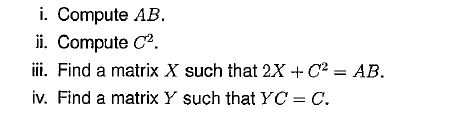
\includegraphics[width=1.11\linewidth]{MatrixQuestion2012}

\end{figure}


%--------------------------------------------%
\noindent \textbf{Part B : Gaussian Elimination - 5 Marks}\\ 
\begin{itemize}
	\item[(i)] Say whether or not the graphs they represent are isomorphic.
	\item[(ii)] Calculate $A^2$ and $A^4$ and say what information each gives about the graph
	corresponding to A. [6]
\end{itemize}
	%===========================================%
	\begin{itemize}
		\item[(i)] Write down the augmented matrix for the following system of equations.
		\[2x + y - z = 2\]
		\[x - y + z = 4\]
		\[x + 2y + 2z = 10\]
		\item[(ii)] Use Gaussian elimination to solve the system. 
	\end{itemize}
%=========================================================================================== %


%-------------------------------------------------------------------------%
\newpage
\end{document}